% !TeX root = ../tesis.tex

%
\begin{figure}[h!]\centering
	\def\svgwidth{.8\textwidth} \small
\includeinkscape{Geometries/SistemaBox}
\vspace*{0em}
\caption[Spherical symmetric COMSOL Setup]{A 3D view (left) and the cross section (right) of a spherical symmetric COMSOL setup to calculate the optical response of a single spherical NP embedded into a matrix. The NP (yellow) is located at the center of the matrix (gray), which is covered by a PML layer (blue). The upper layer of the PML is hidden to allow a better view of the setup.}
\label{fig:setup:sphere}
\end{figure}


%
\begin{figure}[h!]
\def\svgwidth{\textwidth} \small
\hspace*{2em}
\begin{subfigure}{.1\textwidth}\caption{ }\label{fig:Eff:sphere:First:a}\end{subfigure}
\vspace*{12.5em} % Crece la distancia entre as etiquetas
\\
\vspace*{-16.5em} % Crece la distancia entre las etiquetas y el pie de figura
\hspace*{2em}%
\begin{subfigure}{.1\textwidth}\caption{ }\label{fig:Eff:sphere:First:b}\end{subfigure}\\
\includeinkscape{FEM/0-NoConv}
\vspace*{-1.5em} %Crece la ditancia entre la imagen y el pie de figura
\caption[Scattering, Absorption and Extinction Efficiencies of a 5 nm AuNP$@$Air: Analytical and FEM solutions with no optimizatio]{\textbf{a)} Scattering $Q_\text{sca}$, absorption $Q_\text{abs}$ and extinction $Q_\text{ext}$ efficiencies of a 5 nm AuNP embedded into air calculated by means of the Mie Theory (continuous) and the FEM (disks), and \textbf{b)} their absolute error, as function of the wavelength $\lambda$ of the incident plane wave. The chosen parameters for the FEM calculations were based on the COMSOL Excercises \textbf{CITAR}.}
\label{fig:Eff:sphere:First}
\end{figure}


%
\begin{figure}[h!]\centering
	\def\svgwidth{\textwidth} \small
\includeinkscape{FEM/1-Mat-Size-Rad-2}
\vspace*{-1em}
\caption[Extinction Efficiency Absolute Error: NP Max Mesh Size Analysis]{Absolute error between the Mie Theory and the FEM calculation on the extinction efficiency $Q_\text{ext}$ of a 5nm AuNP$@$Air as function of the maximum mesh size within the NP at the wavelength of the LSPR.}
\label{fig:Eff:sphere:radius}
\end{figure}

%
\begin{figure}[h!]\centering
	\def\svgwidth{\textwidth} \small
\includeinkscape{FEM/2-PML-Size}
\vspace*{-1em}
\caption[Extinction Efficiency Absolute Error: Matrix Max Mesh Size Analysis]{Absolute error between the Mie Theory and the FEM calculation on the extinction efficiency $Q_\text{ext}$ of a 5nm AuNP$@$Air as function of the maximum mesh size within the matrix at the wavelength of the LSPR.}
\label{fig:Eff:sphere:matrix}
\end{figure}


\begin{figure}[h!]\centering
	\def\svgwidth{\textwidth} \small
\includeinkscape{FEM/3-Rad-Mesh}
\vspace*{-1em}
\caption[Extinction Efficiency Absolute Error: Matrix and PML Thickness Analysis]{Absolute error between the Mie Theory and the FEM calculation on the extinction efficiency $Q_\text{ext}$ of a 5nm AuNP$@$Air as function of the matrix thickness (black) and the PML thickness (orange) at the wavelength of the LSPR. It wac chosen for both cases a NP maximum mesh size of $a/10$ and a matrix maximum mesh size of $\lambda/6$; the default thickness of the matrix and PML was set to $\lambda/4$.}
\label{fig:Eff:sphere:thickness}
\end{figure}








%
%
%
%\begin{figure}\centering
%%\def\svgwidth{\textwidth} \small
%%\includeinkscape{2-Results-Figs/redshift/redshift}%
%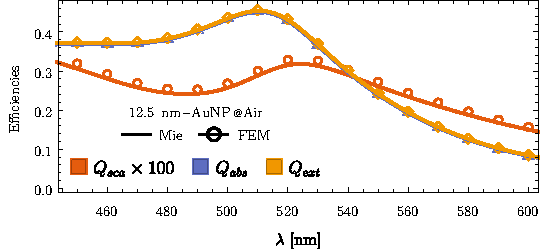
\includegraphics[width = .8\textwidth ]{1-Theory-Figs/Mie-FEM_Air.pdf}\\
%\includegraphics[width = .4\textwidth ]{1-Theory-Figs/Isolated-COMSOL.pdf}%
%\includegraphics[width = .4\textwidth ]{1-Theory-Figs/Isolated-COMSOL.pdf}%
%\caption[Convergence tests: The Meshing]{Resonance wavlength ($\lambda_\text{res}$) of the scattering (orange) and extinction (black) cross sections as functions of the NPs radii when embedded  \ref{sfig:red:1} into air and \ref{sfig:red:2} into water, and as function of the refractive index of the matrix for NP of radius set to  \ref{sfig:red:3} 12.5 nm and \ref{sfig:red:4} 50 nm.}
%\end{figure}




\begin{figure}[h!]\centering
	\def\svgwidth{.8\textwidth} \small
%\includeinkscape{1-Theory-Figs/SistemaBox}
\vspace*{0em}
\caption[Spherical symmetric COMSOL Setup]{A 3D view (left) and the cross section (right) of a spherical symmetric COMSOL setup to calculate the optical response of a single spherical NP embedded into a matrix. The NP (yellow) is located at the center of the matrix (gray), which is covered by a PML layer (blue). The upper layer of the PML is hidden to allow a better view of the setup.}
\label{fig:setup:sphere}
\end{figure}

\begin{figure}[h!]
\def\svgwidth{\textwidth} \small
\hspace*{-1.25em}
\begin{subfigure}{.1\textwidth}\caption{ }\label{fig:Eff:sphere:First:a}\end{subfigure}
\vspace*{12.5em} % Crece la distancia entre as etiquetas
\\
\vspace*{-16.5em} % Crece la distancia entre las etiquetas y el pie de figura
\hspace*{-.75em}%
\begin{subfigure}{.1\textwidth}\caption{ }\label{fig:Eff:sphere:First:b}\end{subfigure}\\
\includeinkscape{FEM/4-Conv}
\vspace*{-1.5em} %Crece la ditancia entre la imagen y el pie de figura
\caption[Scattering, Absorption and Extinction Efficiencies of a 5 nm AuNP$@$Air: Analytical and FEM solutions with no optimizatio]{\textbf{a)} Scattering $Q_\text{sca}$, absorption $Q_\text{abs}$ and extinction $Q_\text{ext}$ efficiencies of a 5 nm AuNP embedded into air calculated by means of the Mie Theory (continuous) and the FEM (disks), and \textbf{b)} their absolute error, as function of the wavelength $\lambda$ of the incident plane wave. The chosen parameters for the FEM calculations were based on the COMSOL Excercises \textbf{CITAR}.}
\label{fig:Eff:sphere:First}
\end{figure}
